% \documentclass[compacto,10pt]{aleph-notas}
\documentclass[compacto,10pt,comentarios]{aleph-notas}

% -- Paquetes adicionales
\usepackage{enumitem}
\usepackage{aleph-comandos}
\usepackage{parskip}
\usepackage{graphicx}
\usepackage{xfrac}
\usepackage{tikz}
\usepackage{etoolbox}
% \AtBeginEnvironment{proof}{\color{white}}
\usepackage[framemethod=tikz]{mdframed}
\DeclareFontFamily{U}{skulls}{}
\DeclareFontShape{U}{skulls}{m}{n}{ <-> skull }{}
\newcommand{\skull}{\text{\usefont{U}{skulls}{m}{n}\symbol{'101}}}
\def \ds{\displaystyle}
\def \dfx{\dfrac{d}{dx}}
\DeclareMathOperator{\arccot}{arccot}
\DeclareMathOperator{\arcsec}{arcsec}
\DeclareMathOperator{\arccsc}{arccsc}

% -- Datos del libro
\institucion{Southwestern College}
\asignatura{MATH 251: Calculus II}
\tema{Surface Area}
\autor{Jesús Pérez Cuarenta}
% \fecha{Fall 2024}

%% --> Logos de las guias
\logouno[4.5cm]{../Images/swc_logo}
\definecolor{colordef}{cmyk}{0.81, 0.62, 0.00, 0.22}

\begin{document}

\encabezado

\section*{Surface Area}
Suppose a curve is given by $y = f(x)$, where $f$ is a function with a continuous first derivative
on the interval $[a, b]$.

Now imagine revolving the curve about the x-axis to generate a surface of revolution.

\begin{figure}[h!]
    \centering
        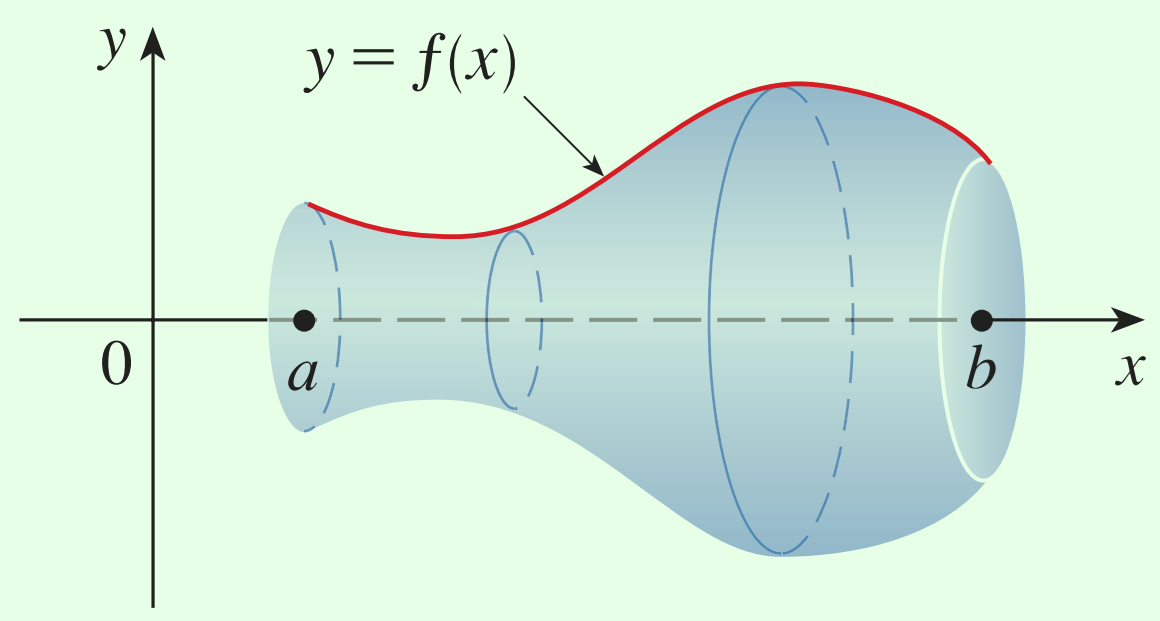
\includegraphics[width=1\linewidth]{../Images/6_6_surfacearea_01.png}
\end{figure}

How can we find the area of this surface?

\begin{defi}[\textbf{Area of a Surface of Revolution}]
    Let $f$ be a nonnegative function with a continuous first derivative on the interval
    $[a, b]$. The area of the surface generated when the graph of $f$ on the interval $[a, b]$
    is revolved about the $x$-axis is
    $$
        S = \int_{a}^{b} 2 \pi f(x) \sqrt{1 + (f'(x))^{2}} ~ dx .
    $$

    Similarly for $x = g(y)$, let $g$ be a nonnegative function with a continuous first derivative on the interval
    $[c, d]$. The area of the surface generated when the graph of $g$ on the interval $[c, d]$
    is revolved about the $y$-axis is
    $$
        S = \int_{c}^{d} 2 \pi g(y) \sqrt{1 + (g'(y))^{2}} ~ dy .
    $$
\end{defi}

%%%%%%%%%%%%%%%%%%%%%%%%%%%%%%%%%%%%%%%%%%%%%%%%%%%%
%% Examples
%%%%%%%%%%%%%%%%%%%%%%%%%%%%%%%%%%%%%%%%%%%%%%%%%%%%
\begin{ejer}
    Find the surface area generated when $y = 2\sqrt{x}$ between $1 \leq x \leq 2$ is rotated about the $x$-axis.
\end{ejer}
\begin{proof}[Solution]
    We have
    $$
        f(x) = 2 x ^{\sfrac{1}{2}} \implies f'(x) = x ^ {-\sfrac{1}{2}}.
    $$
    Applying the definition of surface area for revolving the graph of $f$ about the $x$-axis, we get
    \begin{align*}
        S & = \int_{1}^{2} 2 \pi f(x) \sqrt{1 + (f'(x)) ^ {2}} ~ dx \\
        & = 4 \pi \int_{1}^{2} \sqrt{x} \sqrt{1 + x^{-1}} ~ dx \\
        & = 4 \pi \int_{1}^{2} \sqrt{x} \sqrt{\frac{x + 1}{x}} ~ dx \\
        & = 4 \pi \int_{1}^{2} \sqrt{x + 1} ~ dx .
    \end{align*}
    With $u = x + 1$ and $du = dx$ we arrive at
    \begin{align*}
        4 \pi \int_{1}^{2} (x + 1)^{\sfrac{1}{2}} ~ dx & =  4 \pi \int_{2}^{3} (u)^{\sfrac{1}{2}} ~ du \\
        & = \frac{8\pi}{3} \left. u ^{\sfrac{3}{2}} \right\rvert_{2}^{3} \\
        & = \frac{8\pi}{3} \left( (3)^{\sfrac{3}{2}} - (2)^{\sfrac{3}{2}} \right) \\ 
        & = \frac{8\pi}{3} \left( 3 \sqrt{3} - 2 \sqrt{2} \right).
    \end{align*}
    Therefore,
    $$
    S = \frac{8\pi}{3} \left( 3 \sqrt{3} - 2 \sqrt{2} \right).
    $$
\end{proof}

\begin{ejer}
    The arc of a parabola $y = x ^ {2}$ from $(1, 1)$ to $(2, 4)$ is rotated about the $y$-axis. Find the area of the resulting surface.
\end{ejer}
\begin{proof}[Solution]
    We have
    $$
        g(y) = \sqrt{y} \implies g'(y) = \frac{1}{2} y^{-\frac{1}{2}} = \frac{1}{2\sqrt{y}}.
    $$
    Applying the definition of surface area for revolving the graph of $g$ about the $y$-axis, we get
    \begin{align*}
        S & = \int_{1}^{4} 2 \pi g(y) \sqrt{1 + (g'(y)) ^ {2}} ~ dy \\
        & = 2 \pi \int_{1}^{4} \sqrt{y} \sqrt{1 + \left( \frac{1}{2\sqrt{y}} \right)^{2}} ~ dy \\
        % & = 2 \pi \int_{1}^{4} \sqrt{y} \sqrt{\frac{4y + 1}{4y}} ~ dy \\
        & = 2 \pi \int_{1}^{4} \sqrt{y} \sqrt{1 + \frac{1}{4y}} ~ dy \\
        & = 2 \pi \int_{1}^{4} \sqrt{\left( y \right) \left(1 + \frac{1}{4y} \right)} ~ dy \\
        & = 2 \pi \int_{1}^{4} \sqrt{y + \frac{1}{4}} ~ dy \\
        & = \pi \int_{1}^{4} \sqrt{4y + 1} ~ dy .
    \end{align*}
    With $u = 4y + 1$ and $du = 4 ~ dy$ we arrive at
    \begin{align*}
        \pi \int_{1}^{4} \sqrt{4y + 1} ~ dy & = \frac{\pi}{4} \int_{5}^{17} \sqrt{u} ~ du \\
        & = \frac{\pi}{6} \left(17 \sqrt{17} - 5\sqrt{5} \right) .
    \end{align*}
    Therefore,
    $$
    S = \frac{\pi}{6} \left(17 \sqrt{17} - 5\sqrt{5} \right) .
    $$
\end{proof}

\begin{ejer}
    Set up the integral needed to find the surface area generated by rotating the curve y = $4x - 1$ for $1 \leq x \leq 4$ about the $y$-axis.
\end{ejer}
\begin{proof}[Solution]
    We rewrite $y=4x - 1$ to express $x$ as a function of $y$, say $g(y)$. Note
    $$
        y = 4x - 1 \iff x = \frac{1}{4} \left(y + 1\right).
    $$
    We define $g(y) = \frac{1}{4} (y + 1)$ and apply the definition of surface area for revolving the graph of $g$ about the $y$-axis. Notice
    \begin{align*}
        S & = \int_{3}^{15} 2\pi g(y) \sqrt{1 + \left(g'(y)\right)^{2}} ~ dy \\
        & = \int_{3}^{15} 2 \pi \left(\frac{1}{4}\right) \left( y + 1 \right) \sqrt{1 + \frac{1}{16}} ~ dy \\
        & =  \frac{\pi}{2} \int_{3}^{15} \left( y + 1 \right) \sqrt{\frac{17}{16}} ~ dy \\
        & =  \frac{\sqrt{17}\pi}{8} \int_{3}^{15} \left( y + 1 \right) ~ dy
    \end{align*}
    and we are done.
\end{proof}
\end{document}